% compile with pdflatex and produce svg with pdf2svg
\documentclass[tikz]{standalone}
\usetikzlibrary{arrows.meta,arrows,graphs}
\usetikzlibrary{shapes,decorations,arrows,calc,positioning,automata}
\tikzset{
  edge/.style = {
    semithick
  },
  arc/.style = {
    ->,
    semithick,
    >={[round,sep]Stealth}
  },
  bidir/.style = {
    <->,
    semithick,
    >={[round,sep]Stealth}
  }
}
\begin{document}
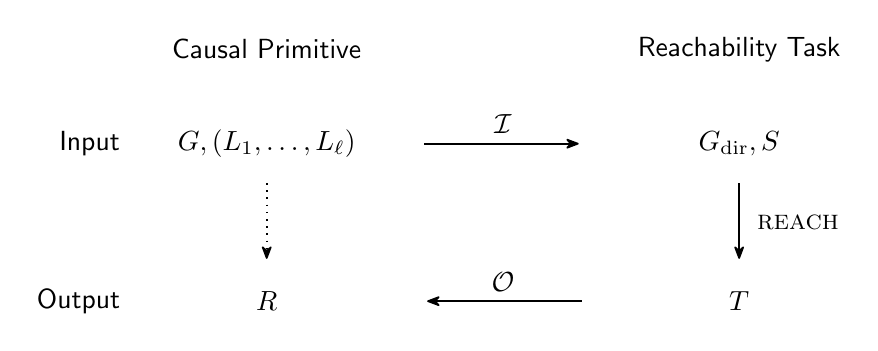
\begin{tikzpicture}
    \node (leftcol)   at (0,-.8) {\textsf{Causal Primitive}};
    \node (rightcol)  at (6,-.8) {\textsf{Reachability Task}};
    \node (upperrow)  at (-2.25,-2) {\textsf{Input}};
    \node (lowerrow)  at (-2.39,-4) {\textsf{Output}};
    \node (causalin)  at (0,-2) {$G, (L_1, \dots, L_{\ell})$};
    \node (causalout) at (0,-4) {$R$};
    \node (reachin)   at (6,-2) {$G_{\mathrm{dir}}, S$};
    \node (reachout)  at (6,-4) {$T$};

    \draw[arc] (2,-2) -- (4,-2) node[midway, above]{$\mathcal{I}$};
    \draw[arc] (6,-2.5) -- (6,-3.5) node[midway, right=0.1cm]{\textsc{reach}};
    \draw[arc] (4,-4) -- (2,-4) node[midway, above]{$\mathcal{O}$};
    \draw[arc, dotted] (0,-2.5) -- (0,-3.5);
\end{tikzpicture}
\end{document}
